\documentclass{amsart}

\usepackage{amssymb}
\usepackage[margin=3cm]{geometry}
\usepackage{epigraph}
\usepackage{natbib}
\usepackage{xcolor}
\usepackage{hyperref}
\usepackage{tikz}

\begin{document}
\pagecolor{white}

\title{Red Queen's Sync Protocol for Ethereum}
\author{Andrew Ashikhmin \& Alexey Akhunov}
\date{April 2019}

\begin{abstract}
    As of early 2019, it takes new Ethereum full nodes a few hours
    to synchronise the blockchain state using eth/63 protocol.
    We propose a new protocol and an algorithm for Ethereum snapshot synchronisation
    that is faster and more robust with respect to the growing state size.
    The new protocol is also tailored towards needs of light clients
    and allows data storage formats other than the canonical Merkle Patricia trie.
    Performance results from a model implementation are encouraging.
\end{abstract}

\maketitle

\epigraph{
    "A slow sort of country!" said the Queen.
    "Now, here, you see, it takes all the running you can do, to keep in the same place.
    If you want to get somewhere else, you must run at least twice as fast as that!"
    }{Lewis Carroll, Through the Looking-Glass and What Alice Found There}

\section{Introduction}

It currently takes new Ethereum full nodes a few hours
to synchronise the blockchain state using eth/63 protocol (\cite{wire_protocol}).
Moreover, the growing state size might potentially result in complete sync failure,
as described in \cite{akhunov_1x_workshop_part1}.

As part of the Ethereum 1x effort, we propose a new sync protocol and algorithm,
which we call Red Queen's.
In our sync algorithm seeders reply with data as of their most recent block.
That results in an inconsistent trie on a leecher initially ("phase 1"),
which is patched later on ("phase 2").
The idea is similar to that of Leaf Sync (\cite{leaf_sync}).
Other sources of inspiration include BitTorrent, Parity's Warp Sync (\cite{warp_sync}),
and Firehose Sync (\cite{firehose}).

Further, we strive to make the protocol work for light clients like Mustekala---see also \cite{light_client_protocol}.

N.B. In this document, we only discuss snapshot synchronisation rather than synchronisation from the Genesis block.

\section{Notation}

We mostly follow the conventions and notations of the Yellow Paper (\cite{yellow_paper}).
For instance, $\mathbb{Y}$ denotes the set of nibble sequences.
We use the letter $\pi$ for prefixes of state or storage trie keys $\mathbf{k} \in \mathbb{B}_{32}$,
\begin{equation}
    \pi \in \mathbb{Y} \; \land \; ||\pi|| \leq 64
\end{equation}
A key matches a prefix if and only if all their first nibbles are the same,
\begin{equation}
    \texttt{MATCH}(\mathbf{k}, \pi) \equiv \forall_{i < ||\pi||}: \mathbf{k}'[i] = \pi[i]
\end{equation}
($\mathbf{k}'$ is a sequence of nibbles, while $\mathbf{k}$ is a sequence of bytes.)

\section{Protocol Specification}

We propose the following new request/reply operative pairs\footnote{For
some extra information see Péter Szilágyi's
\href{https://ethereum-magicians.org/t/forming-a-ring-eth-v64-wire-protocol-ring/2857/10}{comment}
at ETH v64 Wire Protocol Ring.}:\\

\textbf{GetBytecode} (0x20)

[reqID: $\mathbb{N}$,
[codeHash$_0$: $\mathbb{B}_{32}$, codeHash$_1$: $\mathbb{B}_{32}$, ...]]
\medskip

Request EVM code of smart contracts.
The operative is just like $\texttt{GetNodeData}$ from the current version (eth/63) of Ethereum Wire Protocol (\cite{wire_protocol}), except:
\begin{enumerate}
\item includes a request ID;
\item will only return bytecode with the corresponding hash, not arbitrary node data.
\end{enumerate}
\bigskip

\textbf{Bytecode} (0x21)

[reqID: $\mathbb{N}$,
[code$_0$: $\mathbb{B}$, code$_1$: $\mathbb{B}$, ...]]
\medskip

Reply to $\texttt{GetBytecode}$.
Bytecode position in the response list must correspond to the position in the request list;
an empty list $\varnothing$ (i.e. []) should be used for omitted bytecodes.\\

\textbf{GetStateNodes} (0x22)

[reqID: $\mathbb{N}$, blockHash: $\mathbb{B}_{32}$,
[prefix$_0$: $\mathbb{Y}$, prefix$_1$: $\mathbb{Y}$, ...]]
\medskip

Request state trie nodes as of a specific block.
Note that this operative is similar to $\texttt{GetNodeData}$,
but it uses prefixes rather than hashes as node keys\footnote{In
a radix trie there is a trivial one-to-one correspondence between nodes and prefixes.
Since Ethereum employs a modified radix trie with extension nodes,
we define node's prefix as the shortest one such that
all leaves descending from the node match the prefix
and, conversely, all leaves that match the prefix descend from the node in question.}.
It will also only return nodes from the state trie,
not arbitrary node data.
The prefix encoding is described in Appendix C of \cite{yellow_paper}
(no additional flags are utilised).\\

\textbf{StateNodes} (0x23)

[reqID: $\mathbb{N}$,
[node$_0$: $\mathbb{B}$, node$_1$: $\mathbb{B}$, ...],
[availableBlock$_0$: $\mathbb{B}_{32}$, ...]$_{opt}$]
\medskip

Reply to $\texttt{GetStateNodes}$.
An empty list $\varnothing$ returned instead of a node means that the peer does not have enough information about the node requested.
In that case the peer should return blocks for which requested nodes are available
(as a list of $\texttt{availableBlock}$ hashes).

%TODO: Matthew's comment
% Is another way of saying "An empty list returned ... peer does not have enough information ..."
% that the requested data cannot fit in a single response message?
% Or are there other reasons the empty list would be returned?
% If there are multiple reasons it may be worth considering response codes here.

We suggest to use $\texttt{StateNodes}$ primarily to obtain top trie nodes, which will mostly be branch nodes.
Instead of fetching intermediate and bottom nodes with $\texttt{GetStateNodes}$,
we suggest to obtain leaves with $\texttt{GetAccounts}$ operative described below
and build intermediate nodes from subtrie leaves if necessary.
Leaves returned in $\texttt{Accounts}$ contain full 32 byte keys rather than key tails as in leaf nodes.\\

\textbf{GetAccounts} (0x24)

[reqID: $\mathbb{N}$, blockHash: $\mathbb{B}_{32}$, [prefix$_0$: $\mathbb{Y}$, prefix$_1$: $\mathbb{Y}$, ...]]
\medskip

Request state trie leaves (i.e. accounts) as of a specific block
from subtries corresponding to specified prefixes.\\

\textbf{Accounts} (0x25)

[reqID: $\mathbb{N}$,

\quad [

\qquad [status$_0$: $\mathbb{N}$, [[key$^0_{0}$: $\mathbb{B}_{32}$, val$^0_{0}$: $\mathbb{B}$], [key$^1_{0}$: $\mathbb{B}_{32}$, val$^1_{0}$: $\mathbb{B}$], ...]$_{opt}$],

\qquad [status$_1$: $\mathbb{N}$, [[key$^0_{1}$: $\mathbb{B}_{32}$, val$^0_{1}$: $\mathbb{B}$], [key$^1_{1}$: $\mathbb{B}_{32}$, val$^1_{1}$: $\mathbb{B}$], ...]$_{opt}$],

\qquad ...

\quad ],

\quad [availableBlock$_0$: $\mathbb{B}_{32}$, ...]$_{opt}$

]
\medskip

Reply to $\texttt{GetAccounts}$.
Returns accounts that match requested prefixes as key-value pairs\footnote{It
is feasible to return suffixes rather than full keys given that prefixes are known,
but we deem the performance gain to be insignificant.}.
The peer may only return either all leaves of a subtrie or nothing.
$\texttt{status}$ must take one of the following values:
\begin{itemize}
\item 0 -- success;
\item 1 -- no data as of the requested block, the peer should return a list of its available blocks;
\item 2 -- too many leaves matching the prefix.
\end{itemize}
We propose to support up to 4096 leaves per prefix
and return $\texttt{status} = 2$ for bigger subtries.

N.B. The list of available block (hashes) is not specific to a prefix,
but should rather indicate blocks for which most (ideally all) requested prefixes are available.
Also note that state trie replies do not inline storage tries, unlike Leaf Sync.\\

\textbf{GetStorageSizes} (0x26)

[reqID: $\mathbb{N}$, blockHash: $\mathbb{B}_{32}$,
[addressHash$_0$: $\mathbb{B}_{32}$, addressHash$_1$: $\mathbb{B}_{32}$, ...]]
\medskip

Request storage trie sizes as of a specific block.\\

\textbf{StorageSizes} (0x27)

[reqID: $\mathbb{N}$,
[numLeaves$_0$: $\mathbb{N} | \varnothing$, numLeaves$_1$: $\mathbb{N} | \varnothing$, ...],
[availableBlock$_0$: $\mathbb{B}_{32}$, ...]$_{opt}$]
\medskip

Reply to $\texttt{GetStorageSizes}$.
The peer may return an empty list $\varnothing$ instead of the number of leaves for accounts it does not have enough information about.
In that case the peer should return blocks for which requested data is available.

Our sync algorithm does not require precise storage size.
\cite{size_estimation} proposes a fast way of approximate estimation.\\

\textbf{GetStorageNodes} (0x28)

[reqID: $\mathbb{N}$, blockHash: $\mathbb{B}_{32}$,

\quad [addressHash$^0$: $\mathbb{B}_{32}$, [prefix$^0_0$: $\mathbb{Y}$, prefix$^0_1$: $\mathbb{Y}$, ...]],

\quad [addressHash$^1$: $\mathbb{B}_{32}$, [prefix$^1_0$: $\mathbb{Y}$, prefix$^1_1$: $\mathbb{Y}$, ...]],

\quad ...

]
\medskip

Request storage trie nodes as of a specific block.
Similar to $\texttt{GetStateNodes}$.\\

\textbf{StorageNodes} (0x29)

[reqID: $\mathbb{N}$,

\quad [

\qquad [node$^0_0$: $\mathbb{B}$, node$^0_1$: $\mathbb{B}$, ...],

\qquad [node$^1_0$: $\mathbb{B}$, node$^1_1$: $\mathbb{B}$, ...],

\qquad ...

\quad ],

\quad [availableBlock$_0$: $\mathbb{B}_{32}$, ...]$_{opt}$

]
\medskip

Reply to $\texttt{GetStorageNodes}$.
Similar to $\texttt{StateNodes}$.\\

\textbf{GetStorageData} (0x2a)

[reqID: $\mathbb{N}$, blockHash: $\mathbb{B}_{32}$,

\quad [addressHash$^0$: $\mathbb{B}_{32}$, [prefix$^0_0$: $\mathbb{Y}$, prefix$^0_1$: $\mathbb{Y}$, ...]],

\quad [addressHash$^1$: $\mathbb{B}_{32}$, [prefix$^1_0$: $\mathbb{Y}$, prefix$^1_1$: $\mathbb{Y}$, ...]],

\quad ...

]
\medskip

Request storage subtrie leaves as of a specific block.
Similar to $\texttt{GetAccounts}$.\\

\textbf{StorageData} (0x2b)
\nopagebreak

[reqID: $\mathbb{N}$,

\quad [

\qquad [

\quad \qquad [status$^0_0$: $\mathbb{N}$, [[key$^0_{00}$: $\mathbb{B}_{32}$, val$^0_{00}$: $\mathbb{B}$], [key$^0_{01}$: $\mathbb{B}_{32}$, val$^0_{01}$: $\mathbb{B}$], ...]$_{opt}$],

\quad \qquad [status$^0_1$: $\mathbb{N}$, [[key$^0_{10}$: $\mathbb{B}_{32}$, val$^0_{10}$: $\mathbb{B}$], [key$^0_{11}$: $\mathbb{B}_{32}$, val$^0_{11}$: $\mathbb{B}$], ...]$_{opt}$],

\quad \qquad ...

\qquad ],

\qquad [

\quad \qquad [status$^1_0$: $\mathbb{N}$, [[key$^1_{00}$: $\mathbb{B}_{32}$, val$^1_{00}$: $\mathbb{B}$], [key$^1_{01}$: $\mathbb{B}_{32}$, val$^1_{01}$: $\mathbb{B}$], ...]$_{opt}$],

\quad \qquad [status$^1_1$: $\mathbb{N}$, [[key$^1_{10}$: $\mathbb{B}_{32}$, val$^1_{10}$: $\mathbb{B}$], [key$^1_{11}$: $\mathbb{B}_{32}$, val$^1_{11}$: $\mathbb{B}$], ...]$_{opt}$],

\quad \qquad ...

\qquad ],

\qquad ...

\quad ],

\quad [availableBlock$_0$: $\mathbb{B}_{32}$, ...]$_{opt}$

]
\medskip

Reply to $\texttt{GetStorageData}$.
Returns storage data that match requested prefixes as key-value pairs.
The peer may only return either all leaves of a subtrie or nothing.
$\texttt{status}$ values are the same as in $\texttt{Accounts}$.

\section{Suggested Sync Algorithm}

Here we suggest a possible algorithm for full state and storage snapshot synchronisation using the protocol specified above;
light clients are out of scope.
We describe a modus operandi where a seeder replies with its most recent data,
and a leecher has to handle trie data coming from different blocks.
We suggest to perform synchronisation in two stages:
during phase~1 the leecher obtains leaf data\footnote{possibly with necessary proof nodes},
probably as of different blocks,
while during phase~2 it patches up the trie in order to catch up to the most recent block\footnote{The
Red Queen's race is a nice metaphor for phase 2.}.
The idea was proposed in \cite{leaf_sync}.

Let us focus on the state trie for the moment; we shall come back to storage sync later.
For phase~1 we suggest sending $\texttt{GetAccounts}$ requests with a single prefix per request, ditto for phase 2.
All requested prefixes are of size $d_1$ during phase 1 and of $d_2$ during phase 2, $d_2 \geq d_1$.
We elaborate on the values of $d_1$ and $d_2$ later.
The leecher gradually builds the first upper $d_2$ levels of the Merkle Patricia trie\footnote{$d_2$
is small enough so that we can reasonably assume that (almost) all nodes in question are branch nodes;
see \cite{akhunov_1x_workshop_part2}.}.
(The full trie can be constructed if so desired, but only the upper $d_2$ levels are necessary for our algorithm.)
Populated nodes are marked with the block number as of which they are valid.
For simplicity's sake, we assume that all blocks are strictly ordered and ignore chain re-orgs.
The algorithm preserves a following invariant: parent's block is always no older than child's block.

During phase 1 the leecher requests each possible prefix of size $d_1$ exactly once
(barring network failures and faulty peers).
When sending a request,
the leecher sets its $\texttt{blockHash}$ to the latest block.
Having received a reply,
the leecher might choose to verify received leaves by asking for the intermediate nodes ($\texttt{GetStateNodes}$) to the subtrie root.
Then the leecher saves the leaves to the database and updates the nodes along the prefix/path.
By the end of phase 1, the leecher will have all accounts populated, albeit inconsistently.

\begin{figure}[h]
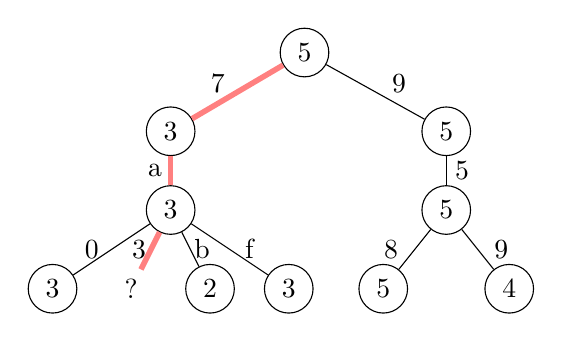
\begin{tikzpicture} [scale=1, auto=left]
\tikzstyle{selected edge} = [draw,line width=2pt,-,red!50]

  \node[circle,draw] (n)       at (4.2,4) {5};
  \node[circle,draw] (n7)     at (2.5,3) {3};
  \node[circle,draw] (n9)     at (6,3)    {5};
  \node[circle,draw] (n7a)   at (2.5,2) {3};
  \node[circle,draw] (n95)   at (6,2)    {5};
  \node[circle,draw] (n7a0) at (1,1)    {3};
  \node(n7a3) at (2,1)    {?};
  \node[circle,draw] (n7ab) at (3,1)    {2};
  \node[circle,draw] (n7af)  at (4,1)    {3};
  \node[circle,draw] (n958) at (5.2,1) {5};
  \node[circle,draw] (n959) at (6.8,1) {4};

  \draw[selected edge] (n) -- (n7);
  \draw (n) -- (n9);
  \draw[selected edge] (n7) -- (n7a);
  \draw (n9) -- (n95);
  \draw (n7a) -- (n7a0);
  \draw[selected edge] (n7a) -- (n7a3);
  \draw (n7a) -- (n7ab);
  \draw (n7a) -- (n7af);
  \draw (n95) -- (n958);
  \draw (n95) -- (n959);
  
  \node at (1.5, 1.5) {0};
  \node at (2.1, 1.5) {3};
  \node at (2.9, 1.5) {b};
  \node at (3.5, 1.5) {f};
  
  \node at (5.3, 1.5) {8};
  \node at (6.7, 1.5) {9};
  
  \node at (2.3, 2.5) {a};
  \node at (6.2, 2.5) {5};
  
  \node at (3.1, 3.6) {7};
  \node at (5.4, 3.6) {9};
\end{tikzpicture}
\setlength{\unitlength}{2cm}
\begin{picture}(1,1)
\put(0.2,0.9){\line(1,0){0.5}}
\put(0.2,1.1){\line(1,0){0.5}}
\put(0.8,1){\line(-1,1){0.2}}
\put(0.8,1){\line(-1,-1){0.2}}
\end{picture}
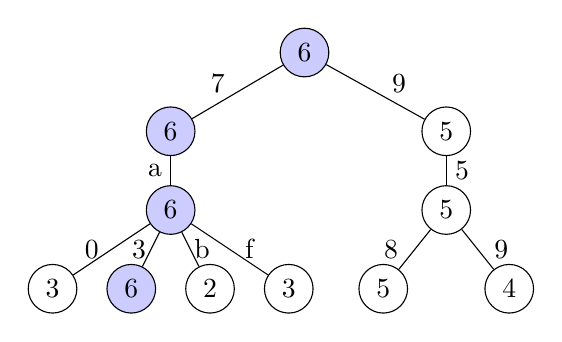
\begin{tikzpicture} [scale=1,auto=left]
  
  \node[circle,draw,fill=blue!20] (n)       at (4.2,4) {6};
  \node[circle,draw,fill=blue!20] (n7)     at (2.5,3) {6};
  \node[circle,draw] (n9)     at (6,3)    {5};
  \node[circle,draw,fill=blue!20] (n7a)   at (2.5,2) {6};
  \node[circle,draw] (n95)   at (6,2)    {5};
  \node[circle,draw] (n7a0) at (1,1)    {3};
  \node[circle,draw,fill=blue!20] (n7a3) at (2,1)    {6};
  \node[circle,draw] (n7ab) at (3,1)    {2};
  \node[circle,draw] (n7af)  at (4,1)    {3};
  \node[circle,draw] (n958) at (5.2,1) {5};
  \node[circle,draw] (n959) at (6.8,1) {4};

  \draw (n) -- (n7);
  \draw (n) -- (n9);
  \draw (n7) -- (n7a);
  \draw (n9) -- (n95);
  \draw (n7a) -- (n7a0);
  \draw (n7a) -- (n7a3);
  \draw (n7a) -- (n7ab);
  \draw (n7a) -- (n7af);
  \draw (n95) -- (n958);
  \draw (n95) -- (n959);
  
  \node at (1.5, 1.5) {0};
  \node at (2.1, 1.5) {3};
  \node at (2.9, 1.5) {b};
  \node at (3.5, 1.5) {f};
  
  \node at (5.3, 1.5) {8};
  \node at (6.7, 1.5) {9};
  
  \node at (2.3, 2.5) {a};
  \node at (6.2, 2.5) {5};
  
  \node at (3.1, 3.6) {7};
  \node at (5.4, 3.6) {9};
\end{tikzpicture}
\caption{Illustration of phase 1 sync. Nodes are labelled with block heights, and edges are labelled with prefix nibbles.}
\label{fig:phase1_example}
\end{figure}

Figure~\ref{fig:phase1_example} shows an example of a phase 1 step with $d_1 = 3$ and $d_2 = 4$.
Say the leecher is interested in prefix $<$7a3$>$.
The trie on the left represents leecher's state before sending a request.
Root's block is 5,
but there is a newer block \#6,
so the leecher sets $\texttt{blockHash}$ accordingly.
After a reply from the seeder,
the leecher saves received leaves to its database and updates the nodes  ($<>$, $<$7$>$, $<$7a$>$, $<$7a3$>$).
The result is displayed on the right of Figure~\ref{fig:phase1_example}.

At the beginning of phase 2, the leecher updates the trie in order to figure out which subtries have to be refreshed
(to the most recent block).
For that, it uses $\texttt{GetStateNodes}$ operative.
The leecher refreshes the trie level by level, starting from the root (level 0) and descending to the level $d_2 - 1$.
Nodes at the same level may be requested in batch.
Having refreshed nodes for a level,
the leecher knows which child nodes one level below have to be refreshed since the leecher can compare their hashes it currently holds with received recent data.
Therefore, only the nodes that have actually changed need to be requested.
The leecher might have to restart the node refresh process from the root if new blocks are mined in between;
however, provided a certain network bandwidth, the process converges.
We analyse convergence conditions in the next section.

When all trie levels from the root down to the level $d_2 - 1$ are up to date,
the leecher knows which nibbles at that last level have changed since phase 1.
It refreshes the leaves corresponding to such nibbles using $\texttt{GetAccounts}$ requests. 
That concludes the algorithm for state trie synchronisation.

The algorithm for storage sync is similar for large storage tries.
Its parameters $d_1$ and $d_2$ are optimised based on the storage size as described in the next section.
$\texttt{GetStorageSizes}$ provides a means of finding out storage sizes.
Small storage tries can be obtained in bulk requesting the empty prefix (meaning the entire trie) for a bunch of them in one go.

\section{Performance Analysis}

In this analysis, we assume that all tries are well balanced.
We also assume that all top nodes up to a certain trie level $i$ are branch nodes, not leaf nor extension nodes.
This is a reasonable assumption if $i$ is not too big---see~\cite{akhunov_1x_workshop_part2}.
Also, we simplify the byte size function of the replies\footnote{Total
request size is much smaller than total reply size, so we ignore requests as well.},
ignoring overheads caused by auxiliary data such as $\texttt{reqID}$,
RLP encoding, and the network layer.
%TODO: internal notation consistency + cross-check against the Yellow Paper
Let us introduce some notation:

$n$ -- the average node size in bytes.
$n$ is essentially equal to the size of a branch node as most nodes transferred are branch nodes.
$n = 530$ is a reasonable estimate.

$l$ -- the average leaf size in bytes, counting both key and value.
For the state trie it is the average account size plus the size of its hash key,
resulting in about 115 bytes.
For storage tries $l \approx 42$.

$t$ -- total number of leaves in a trie.
For the state trie it is the number of accounts,
which is about $53 \cdot 10^6$ as of February 2019---see \cite{akhunov_1x_workshop_part2}.

$b$ -- the network bandwidth available to the leecher.

$\tau$ -- the block time, currently 15 seconds.

$\delta$ -- the average number of leaf changes per block for a trie.
For the state trie it is in the ballpark of 300.

$||R_n||$ -- the number of nodes in a reply $R$ (relevant for $\texttt{StateNodes}$ and $\texttt{StorageNodes}$).

$||R_l||$ -- the number of leaves in a reply $R$ (relevant for $\texttt{Accounts}$ and $\texttt{StorageData}$).

We use the following simplified formula for the byte size of a reply $R$
\begin{equation}
    S(R) = ||R_n|| n + ||R_l|| l
\end{equation}

The overhead of the sync algorithm during phase 1, compared with Parity's warp sync, is in the proof nodes sent alongside the leaf data.
The overhead grows with $d_1$, so we want the trie depth to be as low as possible.
On the other hand, small $d_1$ implies a large number of leaves per reply, which can be brittle or inefficient.
Thus we set $d_1$ to the smallest value possible such that the replies are, on average, no larger than a certain size (say 32 KiB).
We denote that maximum size as $m$.
During phase~1 a $\texttt{Accounts}$ reply
contains $\frac{t}{16^{d_1}}$ leaves on average,
which gives us
\begin{equation}
    \frac{tl}{16^{d_1}} \leq m
\end{equation}
For the state trie the limit of 32 KiB yields $d_1 = 5$.

Let $C(d, \delta)$ be the maximum number of trie nodes from the upper $d$ levels of a trie that can change (on average) per block\footnote{To
be more precise mathematically, $C(d, \delta)$ is an upper bound on the expected value.}.
At each level at most $\delta$ nodes can change, subject to $\delta$ being smaller than the number of nodes at the level.
Thus
\begin{equation}
    C(d, \delta) = \sum_{i=0}^{d-1} \min(16^i, \delta)
\end{equation}
If $16^2 \leq \delta \leq 16^3$ and $d \geq 3$, then
\begin{equation}
    C(d, \delta) = C'(d, \delta) \overset{\underset{\mathrm{def}}{}}{=}
     \delta (d-3) + 273
\end{equation}

We now analyse the minimum bandwidth required for the algorithm to converge during phase 2.
At the very least, "to keep in the same place",
we need to sync all changes per 1 block no slower than the block time $\tau$.
As previously described, the algorithm updates $d_2$ upper levels of the trie.
So the upper bound on the number of nodes to be refreshed is $C(d_2, \delta)$.
The number of subtries that need to be refreshed is no more than $\delta$;
each subtrie has $\frac{t}{16^{d_2}}$ leaves on average.
Summing up, the total reply size per 1 block necessary not to lag behind is no more than
\begin{equation}
    \texttt{RQS} \overset{\underset{\mathrm{def}}{}}{=}
    C(d_2, \delta) \, n + \delta \, \frac{tl}{16^{d_2}}
\end{equation}
(RQS stands for Red Queen's Size).
Though it is an upper bound, for our purposes $\texttt{RQS}$ is close enough to the actual value.
Differentiating, we find the value of $d_2$ that minimises $\texttt{RQS}$
\begin{equation}
    d_2^* = \frac{1}{\ln 16} \ln \left( \frac{tl \ln16}{n} \right)
\end{equation}
(Obviously, one has to round $d_2^*$ up or down.)
For the state trie the optimal $d_2^* = 6$ and the entailing $\texttt{RQS}$ is about 0.7 MiB.
Reiterating, the convergence condition for the state trie alone is
\begin{equation}
    b > \frac{\texttt{RQS}}{\tau}
\end{equation}
For the Ethereum main net as of February 2019 this critical minimum bandwidth is about 0.4 Mbit/s.
Table~\ref{tab:emulated_time} shows the performance results of an emulation of the sync algorithm for various state trie sizes.
The modelling code used is hosted at
\href{https://github.com/yperbasis/silkworm/blob/master/lab/sync_emulator.cpp}{https://github.com/yperbasis/silkworm}.
Network latency was ignored in the emulation.

\begin{table}[h]
\begin{tabular}{ r | c c c }
    Bandwidth & 10M & 50M & 100M \\
    \hline
      1 Mbit/s & 03:39 & 18:44 & 39:04 \\
     10 Mbit/s & 00:20 & 01:39 & 03:17 \\
    100 Mbit/s & 00:02 & 00:10 & 00:20 \\
\end{tabular}
\caption{Emulated times of state trie sync for 10M, 50M, and 100M dust accounts.}
\label{tab:emulated_time}
\end{table}

Convergence analysis for large storage tries (e.g. CryptoKitties) is similar to the state trie analysis above.

\section{Conclusion}

Proposed Red Queen's protocol and algorithm can alleviate slow synchronisation times
caused by the large size of the Ethereum blockchain state.
The protocol is also flexible enough to cater for light clients, not only full nodes.
Our emulation results are promising and corroborate protocol's good scalability and low overhead.
A natural next step forward is to fully implement Red Queen's in a proper Ethereum client
and fledge it into a next version of the standard Ethereum Wire Protocol.

\bibliographystyle{plainnat}
\bibliography{biblio}

\end{document}
